\documentclass{article}


\usepackage{enumitem}
\usepackage{booktabs}
\usepackage{amssymb}
\usepackage{soul}
\usepackage{xspace}
\usepackage{color}
\usepackage{xcolor}
\usepackage{upquote}
\usepackage{listings}
\usepackage{amsmath}
\usepackage{cleveref}
\usepackage{wrapfig}
\usepackage{syntax}

\usepackage{tikz}
\usetikzlibrary{arrows,automata,shapes.misc,shapes.geometric,positioning}


% For comments
\newcommand{\eat}[1]{}
\newcommand{\TODO}[1]{\hl{\textbf{TODO:} #1}\xspace}
\newcommand{\todo}[1]{\hl{#1}\xspace}

%% Bibliography style
\usepackage{booktabs}   %% For formal tables:
                        %% http://ctan.org/pkg/booktabs
\usepackage{subcaption} %% For complex figures with subfigures/subcaptions
                        %% http://ctan.org/pkg/subcaption

\begin{document}

\title{CIS 673 Project Report}
\author{Gautam Mohan and Konstantinos Kallas}


\maketitle

\section{Introduction}

\TODO{Motivate CRDTs and why it makes sense to verify them
  automatically.}

\section{Servois}

\TODO{Describe the technique briefly} \TODO{Describe the tool
  interface. What exactly one has to encode and why}

\section{Conflict Free Replicated Data Types}

\TODO{Fill in with some background information on CRDTs}~\cite{shapiro2011conflict}

\TODO{Say something about both State and Op-based CRDTs.}

\TODO{State correctness conditions Op-based only}

\TODO{Say why we only need to prove commut of effects}

\section{Methodology}

As we mentioned above, in this project we focus on operation based
CRDTs, since proving commutativity of the effects of their supported
operations implies that they are Strongly Eventually Consistent. In
this section, we describe our methodology and informally argue about
its soundness.

In order to encode a data type in Servois, we need to specify (i) its
state, (ii) an equivalence relation on states, (iii) each supported
method (their arguments, preconditions, and postconditions), and (iv)
a set of predicates that can be used by Servois to iteratively refine
the state space. On the other hand, an op-based CRDT specification
contains the following components: (i) a state definition, (ii) a set
of query methods, and (iii) a set of update methods, each of which has
a prepare and an effect method.

We start by encoding the state without any modifications. State
equivalence is defined as a conjunction of the equivalence of all
different state components. Query operations do not be to be encoded
as methods in Servois as they never update the state.
%% \TODO{Check in the CRDT paper if equivalence on states is defined
%%   based on the query methods or based on a complete equivalence of
%%   the states. Accordingly complete this paragraph describing how to
%%   define equivalence.}

We now describe how to encode the update methods. Each update method
has two parts, a \texttt{prepare} and an \texttt{effect}. In Servois
we only encode effects as methods, as we care about how concurrent
updates (that happened in different replicas) can affect the state of
another replica. Intuitively, we want to show that the effects $e_1$,
$e_2$ of two concurrent updates $u_1$, $u_2$ that happened in replicas
$r_1$ and $r_2$ will commute in a third replica $r_3$. In order to
correctly do that, we need to derive preconditions for all the effect
methods by using their prepare methods. More precisely, the
precondition on the arguments of an effect $e$ of an update $u$ that
happened in a replica with state $s'$ must be equivalent to the
postcondition of $u$'s prepare method after it has been applied
$s'$. \TODO{Is that valid?}

\TODO{Figure out what we have to do with effect preconditions. Maybe
  we need to encode them with ite to make sure that if they fail, it
  means that an update is not enabled when it should be?}


Finally, since Servois is sound, i.e. it never concludes that two
methods commute if they don't, we decided to leave the predicates
empty and gradually extend them if we find that Servois is unable to
give an answer \TODO{Check the validity of the above statement by
  reading the Servois paper}.

\TODO{Briefly mention the threats to validity, the fact that we derive
  preconditions based on prepare methods but we don't check them, and
  the fact that we manually encode the postconditions of each method.}

\section{Experience Report}

In this section we describe our experience from proving that several
operation-based CRDTs commute. We briefly describe the semantics of
each CRDT and then explain how we encoded them in the Servois
interface.

\subsection{Last Writer Wins Register}

We first encoded the simple last writer wins register from
\cite{shapiro2011comprehensive}. Its specification is shown in
\Cref{fig:lww-def}. A last writer wins register is a simple register
data type with one value that can be updated and read. It creates a
total order of assignments by associating a unique timestamp with each
update. By always keeping the value with the latest timestamp its
updates commute with each other.

\begin{figure}[h]
    \centering
    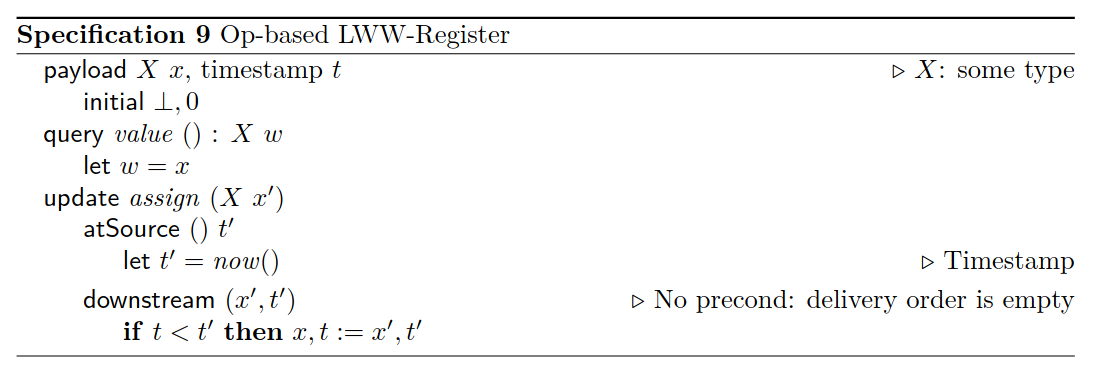
\includegraphics[width=\textwidth]{lww-definition}
    \caption{Last Writer Wins Register}
    \label{fig:lww-def}
\end{figure}

In order to prove that the LWW Register is Strongly Eventually
Consistent, we need to prove that all different concurrent effects
(indicated as ``downstream'' in \cref{fig:lww-def}) commute. Since
only the value $x$ of the register can be returned using queries, we
consider two states to be equivalent if they have the same value $x$.

We started by encoding the state as is (a value $x$ of any type $X$
and a timestamp $t$ of type $Int$) and by encoding the $assign$ effect
by only requiring as a precondition that $t' \neq t$, in order to
enforce timestamp uniqueness. Servois quickly retuned the following
counterexample:

\[
t_1' = t \vee t_2' = t
\]

\TODO{Gautam: Do you understand why exactly does this fail? It is in
  line 36,37 of lwwreg.yml} Servois found that if one of the effect
timestamps $t_1', t_2'$ is equal to the initial timestamp $t$, then
executing them in different orders will lead to one of them not
satisfying the precondition once, but satisfying it in the other
run. However, this behaviour is disallowed by the LWW specification
since all new timestamps $t'$ are unique.

In order to deal with that, we extended the state to keep a set of all
seen timestamps, and we modified the precondition to require that
\TODO{Finish this.}


\TODO{Describe how we implemented it, and why we need to have a set of seen Timestamps to enforce uniqueness.}

\subsection{Grow-only Set and Two-Phase Set}

We have encoded the Grow-only Set (GSet) and Two-Phase Set (2PSet)
from \cite{baquero2017pure}. GSets only support adding items, and they
can be useful when logging events where order is unimportant
(e.g. when storing IPs of clients visiting a web-site). 2PSets extend
GSets by supporting removals, but items that have been removed can
never be added again. Their definitions are shown in
\Cref{fig:gset-def,fig:2pset-def}.

\begin{figure}[h]
    \centering
    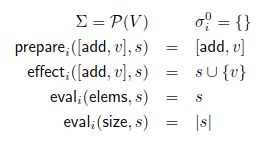
\includegraphics[width=0.5\textwidth]{grow-only-set-definition}
    \caption{Grow-only Set}
    \label{fig:gset-def}
\end{figure}

The state of a GSet is just an originally empty set of values of type
$V$. It's only update function is \texttt{add} which does nothing in
the \texttt{prepare} stage, and then updates the state by inserting
the input element $v$ in the set $s$. The two supported queries are
asking for the elements and the size of the state. The specification
of 2PSet can be seen as a composition of 2 GSets, one for additions
and one for removals. The removals set prohibits items from being
readded to the additions set. 2PSet supports two updating functions,
\texttt{add $v$} and \texttt{remove $v$}. Addition inserts the element
in the addition set only if it doesn't not occur in the removal set,
and removal removes an element from the addition set and adds it in
the removal set. The intuition behind the commutativity of 2PSet is
that removals don't need to happen after an addition to remove the
item, so reversing the order of an addition and a removal of the same
value results in the item being removed.


\begin{figure}[h]
    \centering
    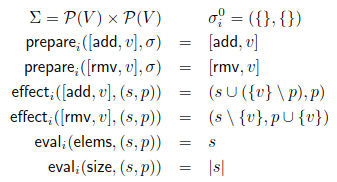
\includegraphics[width=0.5\textwidth]{2pset-definition}
    \caption{Two-Phase Set}
    \label{fig:2pset-def}
\end{figure}

Encoding the two specifications in Servois is mostly straightforward
since all the \texttt{prepare} methods are identity functions without
preconditions. We just encode the result of their effects as
postconditions. Here is an excerpt of the specification of 2PSet,
specifically the state definition and the effect of the \texttt{add}.

\begin{verbatim}
  state:
    - name: Add
      type: (Set V)
    - name: Remove
      type: (Set V)

  methods:
    - name: add
      args:
        - name: v
          type: V
      return:
        - name: result
          type: Bool
      requires: |
        true
      ensures: |
        (and result
             (= Add_new (union (setminus (singleton v) Remove) Add))
             (= Remove_new Remove))
\end{verbatim}

\subsection{Graph CRDTs}

Say some things about the graph in section 5 of
\cite{shapiro2011conflict} and specification 16 from
\cite{shapiro2011comprehensive}.

\TODO{Describe where we got stuck and why.}

%% Bibliography
\bibliography{./draft}
\bibliographystyle{plain}



\end{document}
